% Thanks to http://tex.stackexchange.com/a/30782/5645 for this
% example!
\documentclass{article}
\usepackage{amsmath}
\usepackage{mathptmx}
\usepackage{tikz}
\usepackage{pgfplots}
\usepackage{tkz-fct}
\usetikzlibrary{angles, quotes}
\usetikzlibrary{arrows.meta, arrows}
\usetikzlibrary{external}
\tikzexternalize

\tikzset{
    export as png/.style={
        external/system call/.add={}{
            && convert -density #1 -transparent white "\image.pdf" "\image.png"
        },
    },
    export as png/.default={200},
}

\DeclareSymbolFont{symbolsb}{OMS}{cmsy}{m}{n}
\SetSymbolFont{symbolsb}{bold}{OMS}{cmsy}{b}{n}
\DeclareSymbolFontAlphabet{\mathcal}{symbolsb}
\definecolor{myblue}{rgb}{0.067,0.529,0.871}
\definecolor{mypurple}{rgb}{0.859,0.071,0.525}
\definecolor{myred}{rgb}{1.0, 0.13, 0.32}
\definecolor{mygreen}{rgb}{0.01, 0.75, 0.24}
\definecolor{myblack}{gray}{0.5}
\definecolor{mygray}{gray}{0.7}

\def\req{\protect\rotatebox{90}{$\scriptstyle=$}}

\begin{document}

\tikzset{export as png}

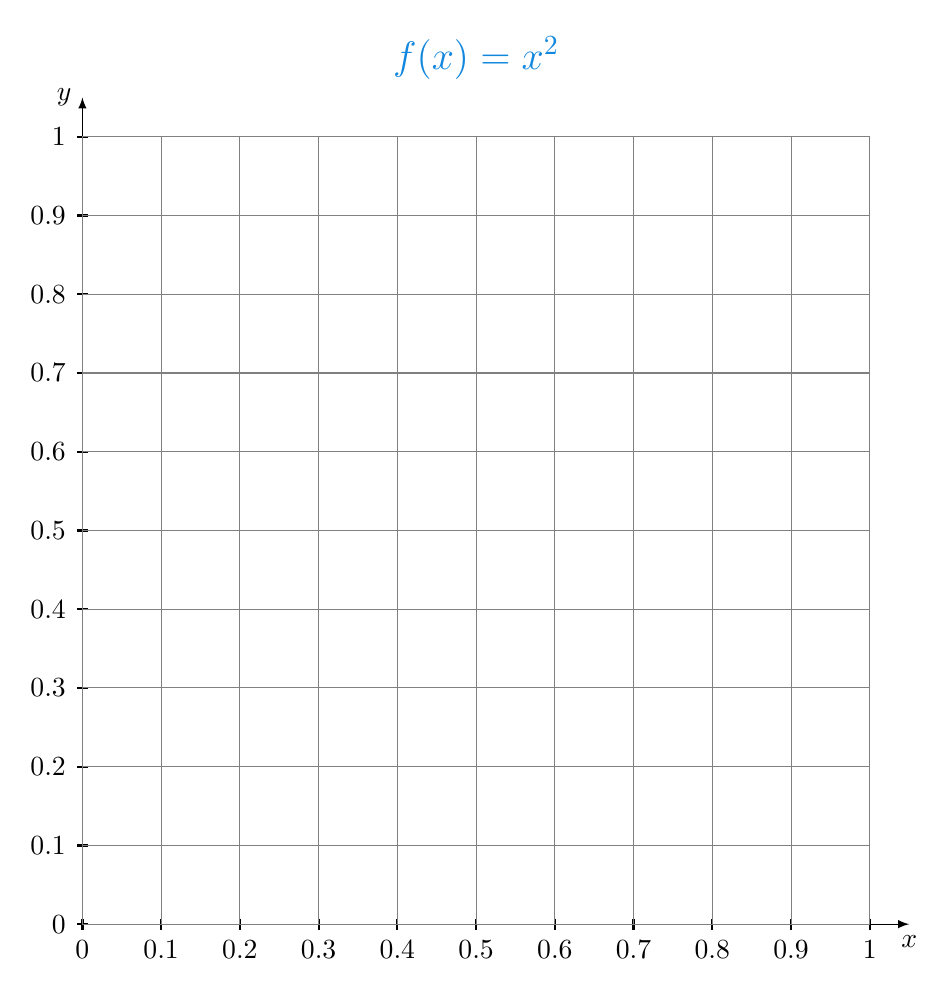
\begin{tikzpicture}[scale=1]
    \tkzInit[xmax=1, ymax=1, xstep=0.1, ystep=0.1]
    \tkzAxeXY
    \tkzGrid
    \tkzFct[line width=1pt, color = myblue]{\x*\x}
    \tkzText(0.5,1.1){\Large $f(x)= x^2$}
\end{tikzpicture}
\end{document}


